%label:"fig:symmetricProductP1"
%parent:""exm:symmetricProductOfP1""
%name:"Symmetric product of $\CP^1$"
%type:"figure"
%caption:"$\CP^2$ can be identified with the 2-fold symmetric product of $\CP^1$. Away from the diagonal, we have symplectic maps."


\usetikzlibrary{decorations.markings}


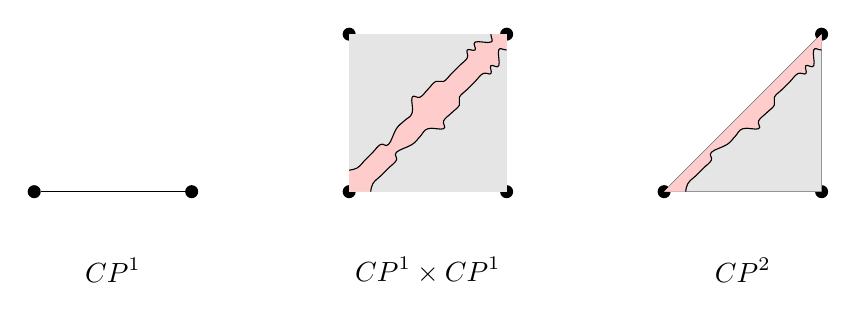
\begin{tikzpicture}


\node[fill=black, circle, scale=.5] (v1) at (0,-1) {};
\node[fill=black, circle, scale=.5] (v2) at (2,-1) {};
\node[fill=black, circle, scale=.5] (v4) at (4,-1) {};
\node[fill=black, circle, scale=.5] (v3) at (4,1) {};
\node[fill=black, circle, scale=.5] (v5) at (6,1) {};
\node[fill=black, circle, scale=.5] (v6) at (6,-1) {};
\node[fill=black, circle, scale=.5] (v7) at (8,-1) {};
\node[fill=black, circle, scale=.5] (v8) at (10,1) {};
\node[fill=black, circle, scale=.5] (v9) at (10,-1) {};
\draw  (v1) edge (v2);
\draw  (v3) edge (v4);
\draw  (v5) edge (v6);
\draw  (v4) edge (v6);
\draw  (v3) edge (v5);
\draw  (v7) edge (v8);
\draw  (v8) edge (v9);
\draw  (v9) edge (v7);
\node at (1,-2) {$\mathbb{CP}^1$};
\node at (5,-2) {$\mathbb{CP}^1\times \mathbb{CP}^1$};
\node at (9,-2) {$\mathbb{CP}^2$};
\fill[gray!20]  (4,1) rectangle (6,-1);
\fill[gray!20] (8,-1) -- (10,1) -- (10,-1);

\begin{scope}[]
\clip (4,-1) -- (4.6,-1) -- (6,0.6) -- (6,1) -- cycle;
\draw[fill=red!20]  plot[smooth, tension=.7] coordinates {(3.8,-1.1) (4.2,-1.1) (4.3,-0.9) (4.4,-0.8) (4.5,-0.7) (4.6,-0.6) (4.6,-0.5) (4.8,-0.4) (4.9,-0.3) (5,-0.2) (5.2,-0.2) (5.2,-0.1) (5.3,0) (5.4,0.1) (5.4,0.2) (5.5,0.3) (5.6,0.4) (5.7,0.5) (5.8,0.5) (5.8,0.6) (5.9,0.6) (5.9,0.8) (6,0.8) (6.2,0.8) (6.2,1) (5.9,1.2)};

\end{scope}

\begin{scope}[xscale=-1, rotate=90, shift={(-5,5)}]
\clip (4,-1) -- (4.6,-1) -- (6,0.6) -- (6,1) -- cycle;
\draw[fill=red!20]  plot[smooth, tension=0.7] coordinates {(3.8,-1.1) (4.2,-1.1) (4.3,-0.9) (4.4,-0.8) (4.5,-0.7) (4.6,-0.6) (4.6,-0.5) (4.8,-0.4) (4.9,-0.3) (5,-0.2) (5.2,-0.2) (5.2,-0.1) (5.3,0) (5.4,0.1) (5.4,0.2) (5.5,0.3) (5.6,0.4) (5.7,0.5) (5.8,0.5) (5.8,0.6) (5.9,0.6) (5.9,0.8) (6,0.8) (6.2,0.8) (6.2,1) (5.9,1.2)};

\end{scope}

\begin{scope}[shift={(4,0)}]
\clip (4,-1) -- (4.6,-1) -- (6,0.6) -- (6,1) -- cycle;
\draw[fill=red!20]  plot[smooth, tension=0.7] coordinates {(3.8,-1.1) (4.2,-1.1) (4.3,-0.9) (4.4,-0.8) (4.5,-0.7) (4.6,-0.6) (4.6,-0.5) (4.8,-0.4) (4.9,-0.3) (5,-0.2) (5.2,-0.2) (5.2,-0.1) (5.3,0) (5.4,0.1) (5.4,0.2) (5.5,0.3) (5.6,0.4) (5.7,0.5) (5.8,0.5) (5.8,0.6) (5.9,0.6) (5.9,0.8) (6,0.8) (6.2,0.8) (6.2,1) (5.9,1.2)};

\end{scope}

\end{tikzpicture}